\section{Background Theory}

	\subsection{Classification of Graphical Passwords}

    A varity of graphical passwords schemes have been created over the past years. Biddle et al. have collected research 
    of the past decade on graphical password schemes \cite{Biddle}, dividing the schemes into three categories: recall-based, 
    recognition-based, and cued-recall authentication. 

    \subsection*{Recall-based}
      Recall-based graphical passwords are often referred to as drawmetric systems \cite{DeAngeli} because the user are
      are reproducing a secret drawing. The password is normally drawn in a grid or a blank canvas, requireing the
      user to reproduce the secret password from its memory.
      Some of the known recall-based password schemes are Pass-Go and Draw-a-secret (DAS).

      \begin{figure}[H]
        \centering
        \subfigure{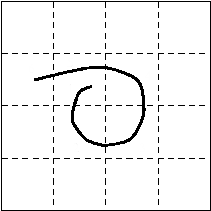
\includegraphics[scale=0.70]{pics/DAS.png}}
        \subfigure{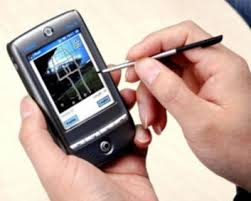
\includegraphics[scale=0.73]{pics/BDAS.jpg}}
        \caption{1) DAS 2)DAS with background}
      \end{figure}

        
    \subsection*{Recognition-based}
      Recognition-based passwords are often referred to as cognometric systems \cite{DeAngeli} because the user recall 
      a secret drawing, or sequence of drawings, and the reproduces it as the secret password. Example of implemented 
      recognition-based password schemes are `Passface' and `Deja vu' that uses a sequence of user selected faces/images as a authentication code.

      \begin{figure}[H]
        \centering
        \subfigure{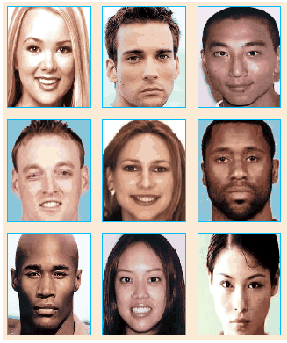
\includegraphics[scale=0.49]{pics/Passface.png}}
        \subfigure{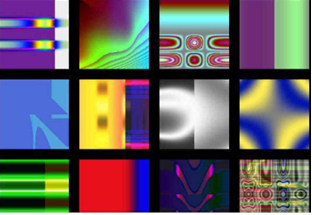
\includegraphics[scale=0.77]{pics/DejaVu.png}}
        \caption{1) Passface 2) Deja vu}
      \end{figure}

    \subsection*{Cued-recall}
      Cued-recall are often referred to locimetric systems \cite{DeAngeli}. With cued-recall authentication typically 
      require the users to remember and target a specific location within and image. This is a version of a recall-based 
      authentication, but helps the user with the recall by showing an image and not just an grid or canvas. It is allso 
      different from the recognition-based approah becuase the user need to indentify spesific locations in an image as a whole. 
      One of the known Cued-Recall password scheme are PassPoints.

      \begin{figure}[H]
        \centering
        \subfigure{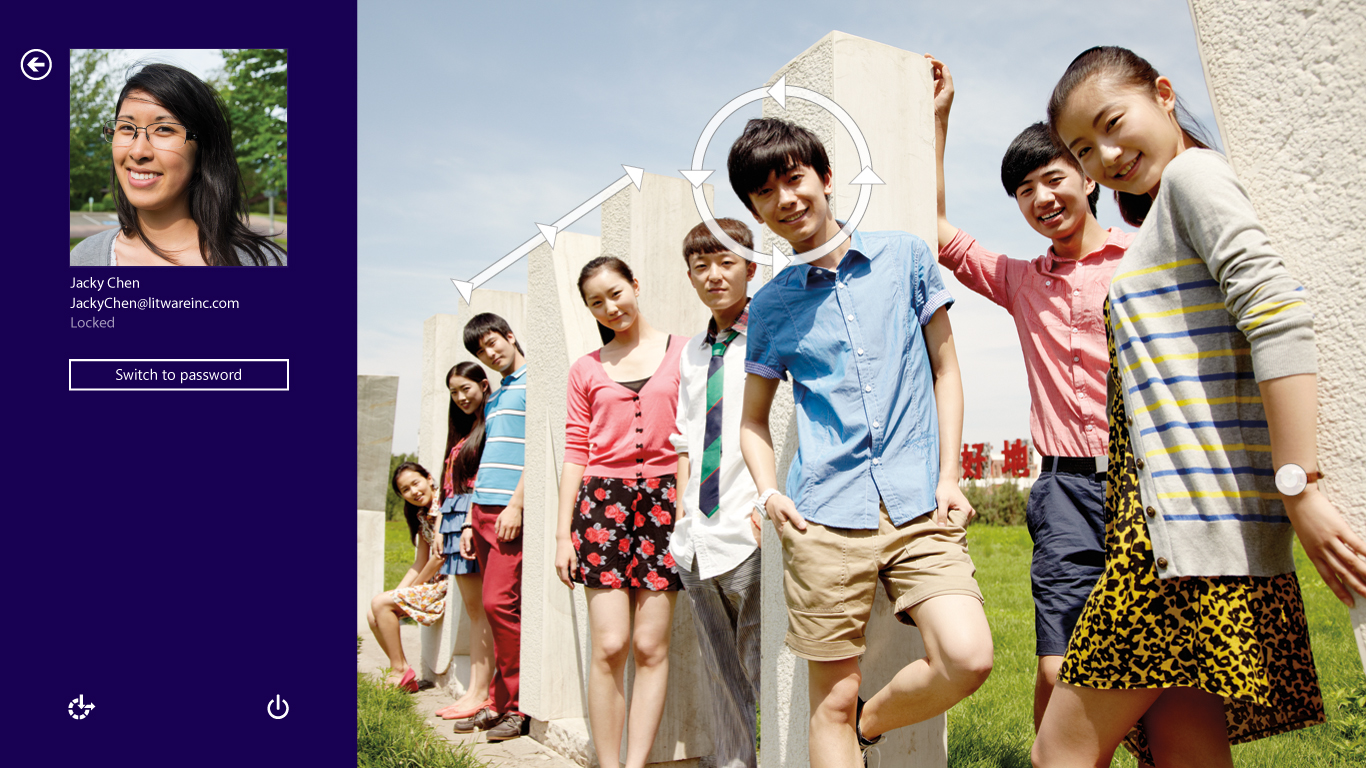
\includegraphics[scale=0.24]{pics/Passpoint.jpg}}
        \caption{1) Passpoints}
      \end{figure}

  
  \clearpage
  \subsection{Android Unlock Pattern}

    % When was the first unlock pattern made
    % Hvorfor er dette en standard for bare android og ikke ios?

    The Android Unlock Patterns are a simplified version of the Pass-Go scheme that was proposed by 
    Tao and Adams in 2008, and can be seen as a successor of the Draw-a-Secret (DAS) scheme.
    Both Pass-Go, Draw-a-Secret, and Android Unlock Patterns is categorized as recall-based authentication schemes.

    The Android password patterns are a simplified version of the Pass-Go scheme using a 3x3 grid, instead of a 9x9 as 
    the Pass-Go scheme originally was designed. The Pass-Go scheme was inspiered from the chineese board game ``Go''.

    The settings on Android phones provides a default setting for using the Unlock pattern. 
    The rules are simple: 
        \begin{enumerate}
            \item At least four points must be chosen,
            \item You cannot vist the same node twice.
            \item Only straight lines are allowed, and
            \item One cannot jump over point not visited before
        \end{enumerate}

    \begin{figure}[H]
        \centering
        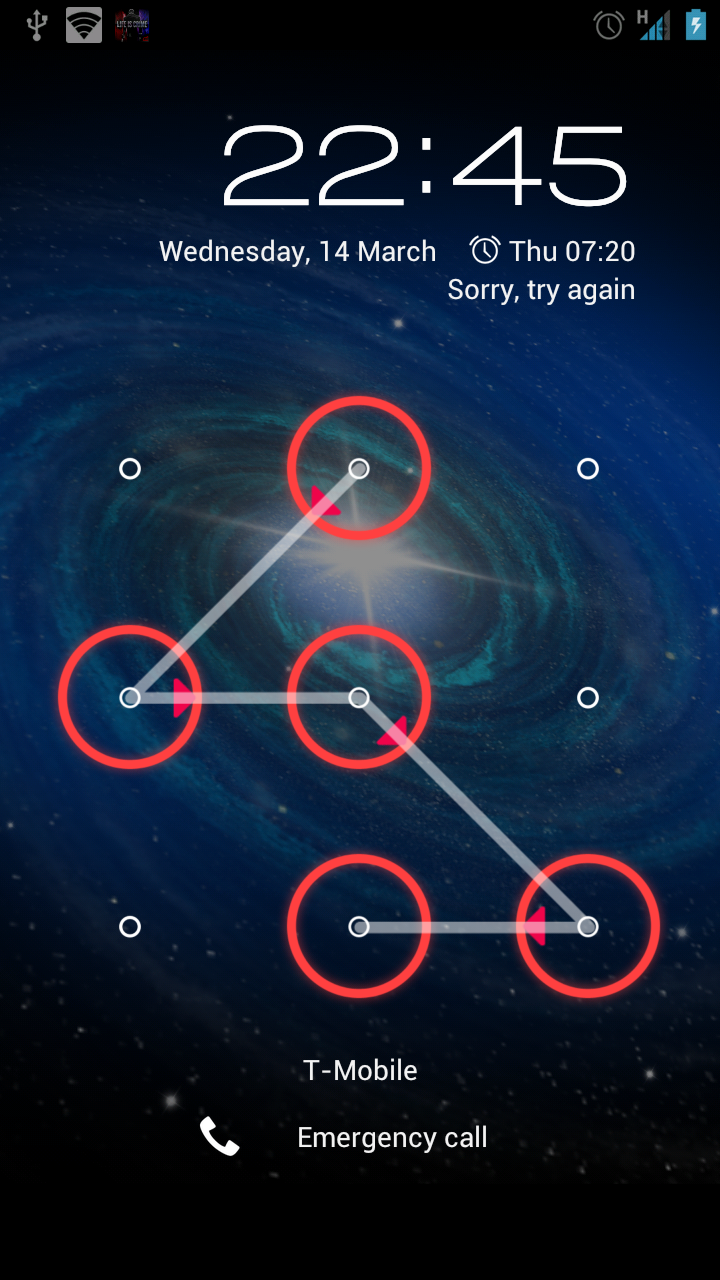
\includegraphics[scale=0.8]{pics/patternLock.png}
    \end{figure}


 %  \section{Passphrase and PIN's vs. graphical passwords}
 %  \section{A password are more then just a password}

 %    If you take a walk in the street and ask a random person ``what is a password?'', 
 %    you probably get the aswer ``its letters and digits''. Passwords are so much more than just letter and digits. 

 %    Nowadays everything we do require you to keep this secret called a password. Your work, you're social life, 
 %    even you're private life is forcing you to keep track of passwords. How do you keep track of all of them?
 %    You probably keep the same password at many places. 
 %    \subsection{Theoretical Password Space}
 %    \subsection{Practical Password Space}

 %  \section{Relevant Data Collection Methods}
 %    In this section I will explore different methods for collecting data. It will give a brief summary of the 
 %    method as well as summary and discussion of the different methods at the end. 
 %    \subsection{Android Unlock Patterns Games}
 %    \subsection{Relevant User Studies}
 %    \subsection{Summary of Methods}
 %  \section{Information gathering}
	% \section{Psycology and passwords}
	% \section{Graphical passwords}
	% \section{Android Unlock Pattern}
